\section {Assessments}
Since the presentation, logic and data layer was implemented by other thesis team mates, only the libraries and user interface design will be mentioned for the Assessments feature.

\subsection{Libraries used}
The following libraries were used for the Assessment feature:

\begin{enumerate}
	\item React Router - a library used for routing and navigation between components in ReactJS. It allows passing data and navigation between components a lot cleaner and simpler.
	\item Chakra UI - A UI library that is simple, easy to use and provides a visually appealing interface. 
\end{enumerate}

\subsection{User Interface Design}
The user interface is what the user relies on to complete tasks and thus it is important that the design is usable and easy to use. A few changes were made from the initial designs to support the added content that was not planned in earlier stages of the Assessments feature. A more detailed insight of the user interface is shown in the Walkthrough chapter under the Assessments section. 

\subsubsection{Final Designs}
The final design had more emphasis on possible tools that'd improve the user experience and was added to reduce the amount of time the user needs to spend on their tasks: 

\begin{enumerate}
	\item Quiz Creation page: contains the questions list and the expand/collapse functionality to allow the user to focus on particular questions
	\item Quiz Usage page: contains the quiz progression column that allows them to keep track of which questions they've attempted or not attempted as well as the ability to navigate to any question with one click
	\item Quiz Review Submission page: highlights incorrect answers vs. the correct answers and shows all explanations (that were provided by the quiz creator) for the possible answers
\end{enumerate}

\begin{figure}[h!]
	\centering
	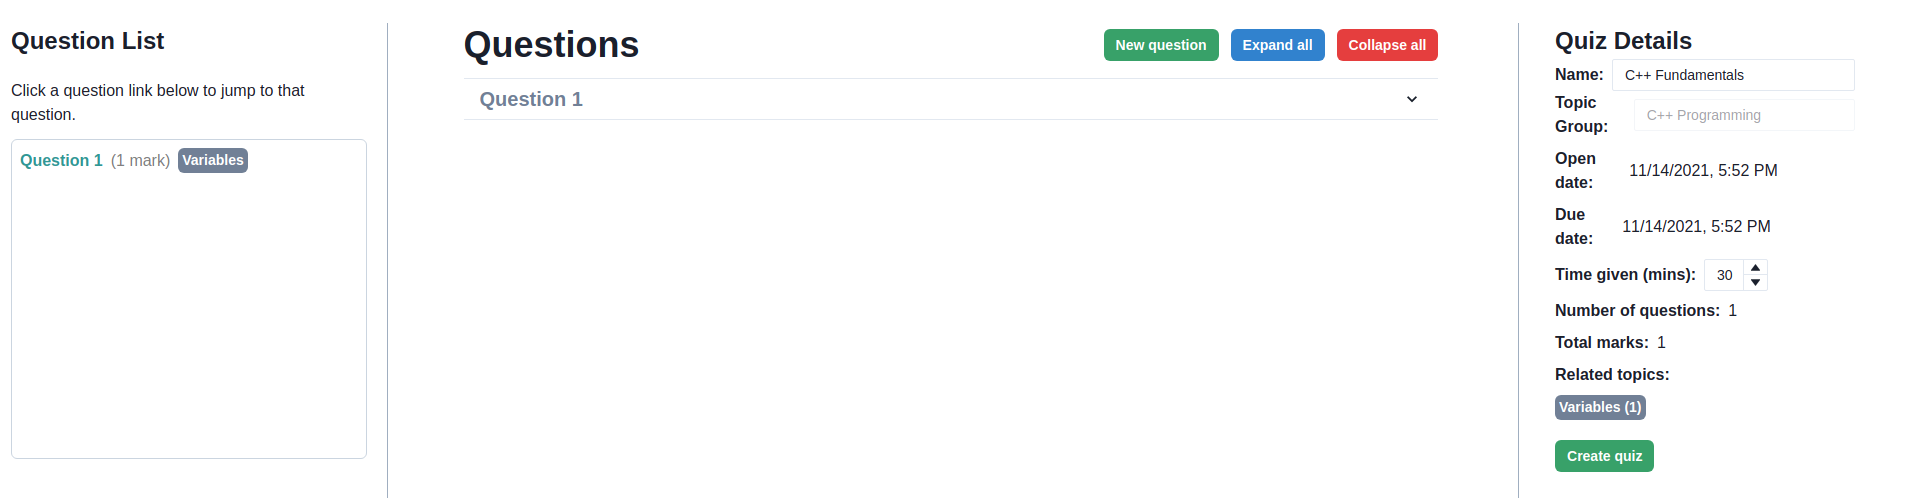
\includegraphics[scale=0.35]{assessments-question-list}
	\caption{Quiz creation page}
\end{figure}

\begin{figure}[h!]
	\centering
	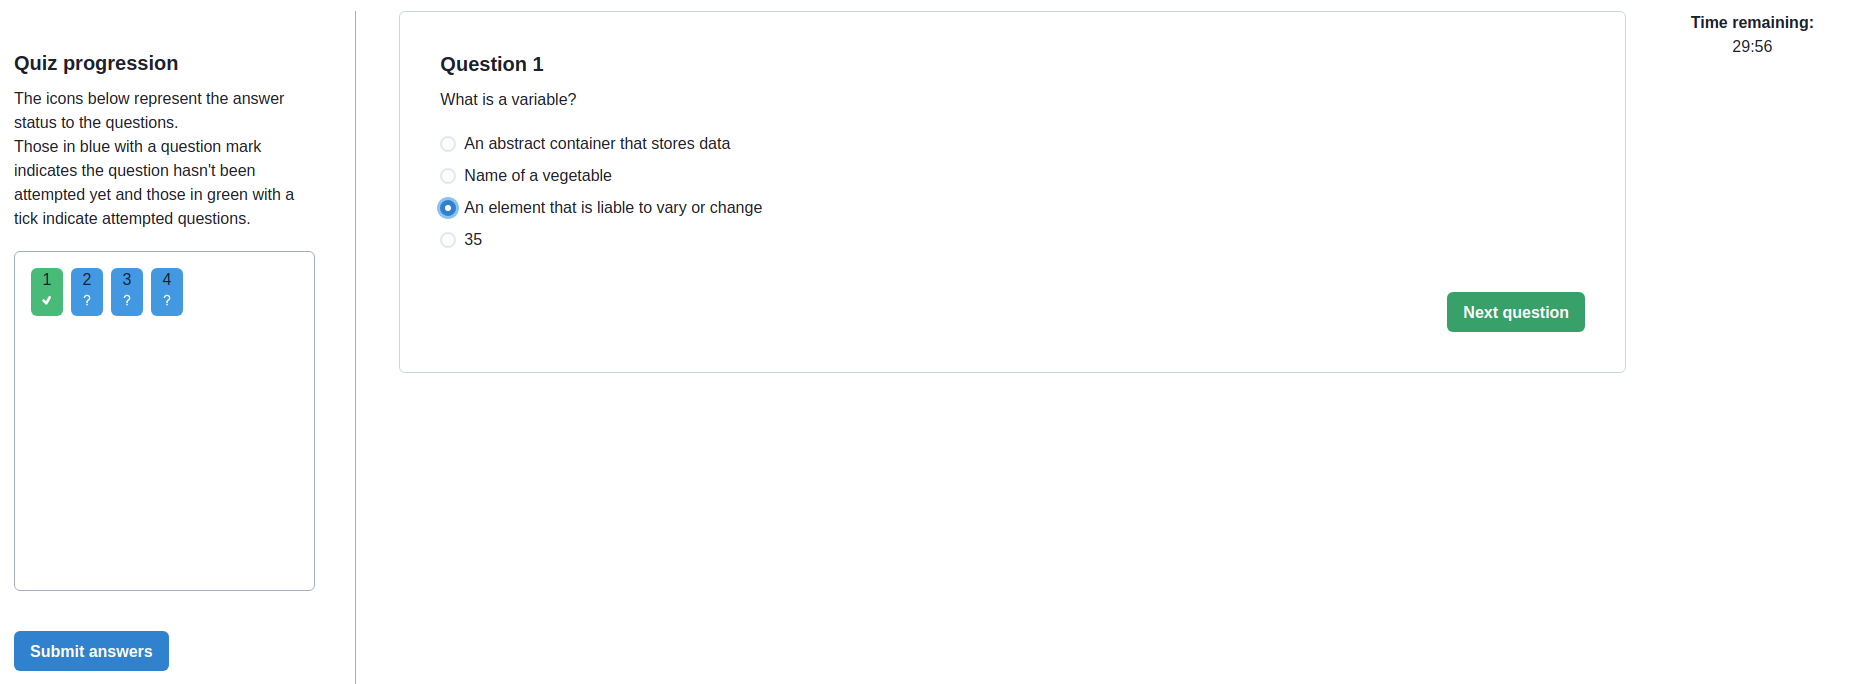
\includegraphics[scale=0.35]{assessments-quiz-usage-interface}
	\caption{Quiz usage page}
\end{figure}

\begin{figure}[h!]
	\centering
	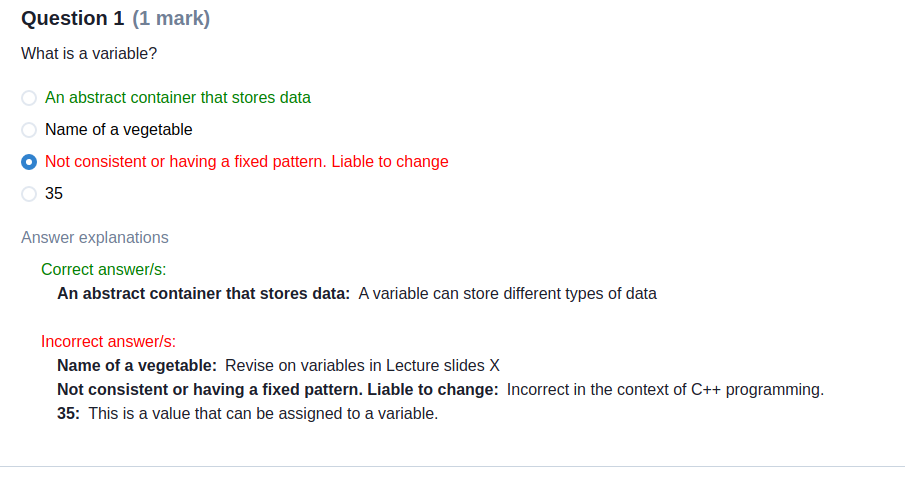
\includegraphics[scale=0.35]{assessments-view-submission}
	\caption{Quiz review submission page}
\end{figure}


\subsubsection{Changes Made From Initial Designs}
There were significant changes to the initial designs in terms of button layouts and colour schemes, however the core content displayed is the same. Additional data that was not foreseen or thought of during initial designing was added to the user interface design. Furthermore, extra tools were added for convenience and to improve the user experience. 

Below, the initial and final designs next to each other to see the similarities and differences.

Question creation:

\begin{figure}[h!]
	\centering
	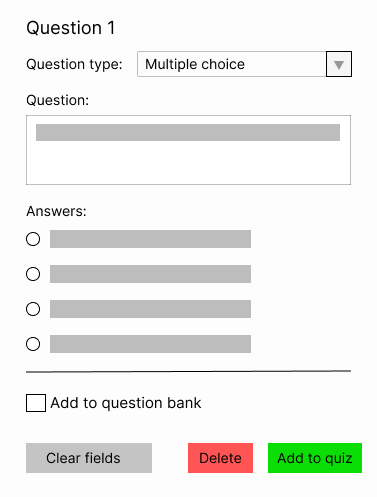
\includegraphics[scale=0.35]{assessments-quiz-creation}
	\caption{Initial design of question creation}
\end{figure}

\begin{figure}[h!]
	\centering
	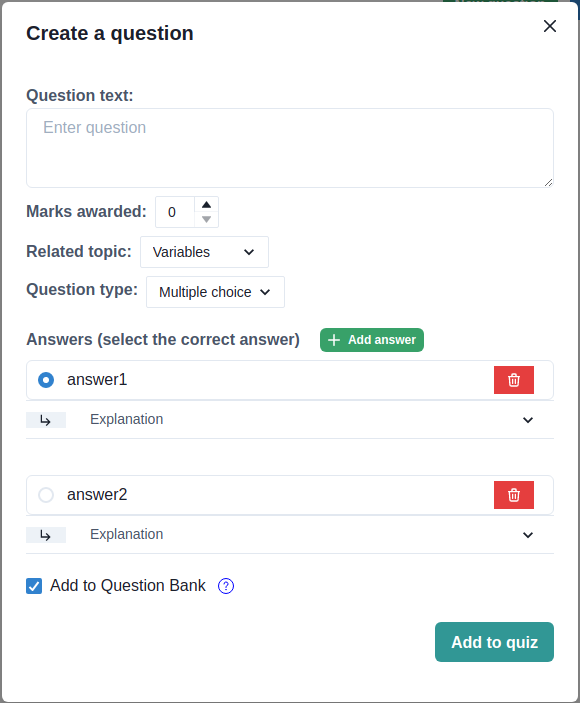
\includegraphics[scale=0.35]{assessments-new-question-modal}
	\caption{Final design of question creation}
\end{figure}


Quiz usage:

\begin{figure}[h!]
	\centering
	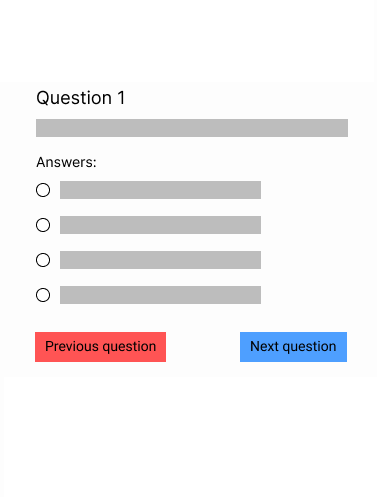
\includegraphics[scale=0.35]{assessments-quiz-usage}
	\caption{Initial design of quiz usage}
\end{figure}

\begin{figure}[h!]
	\centering
	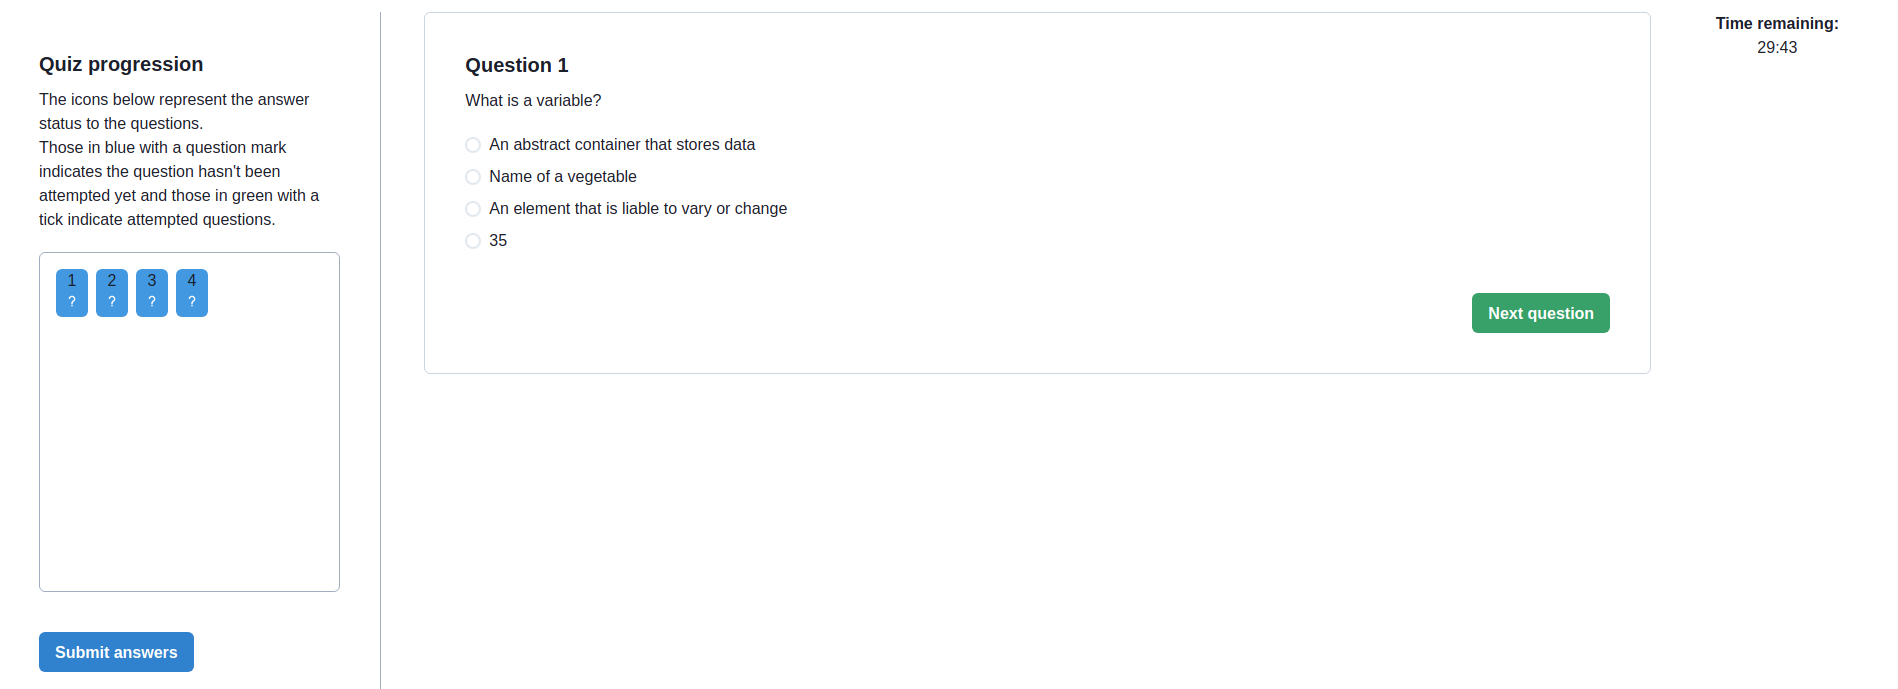
\includegraphics[scale=0.25]{assessments-quiz-submission}
	\caption{Final design of quiz usage}
\end{figure}